\documentclass[a4paper]{article}

\usepackage[utf8]{inputenc}
\usepackage[portuges]{babel}
\usepackage{indentfirst}
\usepackage{graphicx}
\usepackage{float}
\usepackage{caption}
\usepackage{subcaption}
\usepackage[T1]{fontenc}
\usepackage{listings}
\usepackage{amsmath}
\usepackage{mathtools}
\renewcommand{\familydefault}{\sfdefault}

\title{Projeto de Computação Gráfica - Fase 1}
\author{Diogo Braga A82547 \and João Silva A82005 \and Ricardo Caçador A81064
\and Ricardo Veloso A81919}
\date{\today}

\begin{document}

\maketitle

\begin{abstract}
Neste relatório é apresentada a primeira fase dum projeto no qual a intenção é desenvolver um mecanismo 3D baseado em gráficos de cenas e fornecer exemplos de uso que mostrem o seu potencial, desenvolvido no âmbito da unidade curricular de Computação Gráfica.
\end{abstract}

\tableofcontents

\newpage


\section{Introdução}
\label{sec:intro}

Esta primeira fase tem como objetivo a criação de duas aplicacões: \textit{generator} e \textit{engine}.
(...)

\section{Generator}
\label{sec:generator}

\subsection{Explicação dos ficheiros criados}
\label{sec:ficheiros}

Cada função recebe como último parâmetro uma string com o nome do ficheiro que vai guardar os pontos que constituem os triângulos necessários para a criação de cada figura.

(...)

\subsection{\textit{Plane}}
\label{sec:plane}
A função \textit{generatePlane} recebe como parâmetro um float que representa o comprimento de cada lado do plano (side).

(...)

\ttfamily
\begin{enumerate}
  \item Atribuir à variavel parcial\_side o valor de side/2
  \item Construir o primeiro triângulo com os pontos:

        \hspace{2cm} P1 $\Rightarrow$ (parcial\_side, 0.0, -parcial\_side)

        \hspace{2cm} P2 $\Rightarrow$ (-parcial\_side, 0.0, -parcial\_side)

        \hspace{2cm} P3 $\Rightarrow$ (-parcial\_side, 0.0, parcial\_side)
  \item Construir o segundo triângulo com os pontos:

        \hspace{2cm} P1 $\Rightarrow$ (parcial\_side, 0.0, -parcial\_side)

        \hspace{2cm} P2 $\Rightarrow$ (-parcial\_side, 0.0, parcial\_side)

        \hspace{2cm} P3 $\Rightarrow$ (parcial\_side, 0.0, parcial\_side)
  \item Fim
\end{enumerate}
\rmfamily


\subsection{\textit{Box}}
\label{sec:box}
A função \textit{generateBox} recebe como parâmetro três floats que representam as dimensões de cada eixo da caixa (X, Y e Z), e um inteiro que representa o número de divisões que a caixa tem. (???????????????)

(...)

\subsection{\textit{Sphere}}
\label{sec:sphere}

\newpage

\subsection{\textit{Cone}}
\label{sec:cone}
A função \textit{generateCone} recebe como parâmetro um float que representa o raio da base do cone, um float que representa a altura do cone, um inteiro que representa o número de triângulos que queremos que constituam a base, e ainda outro inteiro que representa o número de \textit{stacks} que constituem o lado do cone.


% figura

\ttfamily
$$\alpha_{1} = slice\_atual \times \frac{2\pi}{numero\_slices} $$

\vspace{0.5cm}

$$\alpha_{2} = (slice\_atual+1) \times \frac{2\pi}{numero\_slices} $$

\vspace{0.5cm}

        \hspace{1.5cm} P1 $\Rightarrow$ (raio $\times$ cos($\alpha_{1}$) , 0.0, raio $\times$ sin($\alpha_{1}$))

\vspace{0.2cm}

        \hspace{1.5cm} P2 $\Rightarrow$ (raio $\times$ cos($\alpha_{2}$) , 0.0, raio $\times$ sin($\alpha_{2}$))

\vspace{0.2cm}

        \hspace{1cm} P1' $\Rightarrow$ (raio' $\times$ cos($\alpha_{1}$) , height, raio' $\times$ sin($\alpha_{1}$))

\vspace{0.2cm}

        \hspace{1cm} P2' $\Rightarrow$ (raio' $\times$ cos($\alpha_{2}$) , height, raio' $\times$ sin($\alpha_{2}$))

\rmfamily

\newpage

\subsubsection{Algoritmo:}

\ttfamily
\begin{enumerate}
  \item Iterar sobre o número de slides:
  \begin{enumerate}
    \item Calcular o ângulo $\alpha$ para o slice atual $\Rightarrow$ \underline{$\alpha_{atual}$}
    \item Calcular o ângulo $\alpha$ para o slice seguinte $\Rightarrow$ \underline{$\alpha_{seguinte}$}
    \item Construir os pontos do triângulo formado pelas duas slices atuais:

    \vspace{0.5cm}

        \hspace{3cm} P1 $\Rightarrow$ (0.0, 0.0, 0.0)

    \vspace{0.2cm}

        \hspace{1cm} P2 $\Rightarrow$ (raio $\times$ cos($\alpha_{atual}$) , 0.0, raio $\times$ sin($\alpha_{atual}$))

    \vspace{0.2cm}

        \hspace{0.5cm} P3 $\Rightarrow$ (raio $\times$ cos($\alpha_{seguinte}$) , 0.0, raio $\times$ sin($\alpha_{seguinte}$))

    \vspace{0.3cm}

    \item Guardar altura atual para usar na seguinte iteração $\Rightarrow$ \underline{ph}
    \item Guardar raio atual para usar na seguinte iteração $\Rightarrow$ \underline{pr}

    \item Iterar sobre o número de stacks exceto a última:
    \begin{enumerate}
      \item Calcular a altura da stack atual $\Rightarrow$ \underline{nh}
      \item Calcular o raio da stack atual $\Rightarrow$ \underline{nr}
      \item Construir os dois triângulos da stack atual:

      \vspace{0.5cm}

      \underline{Primeiro triângulo:}

      \vspace{0.5cm}

          \hspace{0.5cm} P1 $\Rightarrow$ (nr $\times$ cos($\alpha_{atual}$) , nh, nr $\times$ sin($\alpha_{atual}$))

      \vspace{0.2cm}

          \hspace{0.5cm} P2 $\Rightarrow$ (pr $\times$ cos($\alpha_{seguinte}$) , ph, pr $\times$ sin($\alpha_{seguinte}$))

      \vspace{0.2cm}

          \hspace{0.5cm} P3 $\Rightarrow$ (pr $\times$ cos($\alpha_{atual}$) , ph, pr $\times$ sin($\alpha_{atual}$))

      \vspace{0.5cm}

      \underline{Segundo triângulo:}

      \vspace{0.5cm}

          \hspace{0.5cm} P1 $\Rightarrow$ (nr $\times$ cos($\alpha_{atual}$) , nh, nr $\times$ sin($\alpha_{atual}$))

      \vspace{0.2cm}

          \hspace{0.5cm} P2 $\Rightarrow$ (nr $\times$ cos($\alpha_{seguinte}$) , nh, nr $\times$ sin($\alpha_{seguinte}$))

      \vspace{0.2cm}

          \hspace{0.5cm} P3 $\Rightarrow$ (pr $\times$ cos($\alpha_{seguinte}$) , ph, pr $\times$ sin($\alpha_{seguinte}$))

      \vspace{0.3cm}
    \end{enumerate}

    \item Construir o triângulo da ponta do cone (última stack), formado pelos pontos:

    \vspace{0.5cm}

        \hspace{3cm} P1 $\Rightarrow$ (0.0, height, 0.0)

    \vspace{0.2cm}

        \hspace{0.5cm} P2 $\Rightarrow$ (pr $\times$ cos($\alpha_{seguinte}$) , ph, pr $\times$ sin($\alpha_{seguinte}$))

    \vspace{0.2cm}

        \hspace{1cm} P3 $\Rightarrow$ (pr $\times$ cos($\alpha_{atual}$) , ph, pr $\times$ sin($\alpha_{atual}$))

    \vspace{0.3cm}

  \end{enumerate}

  \item Fim
\end{enumerate}
\rmfamily

\newpage

\section{Engine}
\label{sec:engine}
De forma a representar as figuras de uma determinada cena, usou-se XML para referenciar os ficheiros “.3d” construídos pelo gerador. Esses ficheiros contêm várias pontos que dão resultado a vários triângulos, que resultam em figuras.

\begin{figure}[H]
\centering
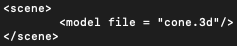
\includegraphics[scale=0.70]{scene_xml.png}
\caption{Exemplo "scene.xml"}
\label{img:scene}
\end{figure}

\section{Câmera}
\label{sec:camera}
De forma a poder visualizar as figuras de diferentes ângulos criamos uma câmera que pode variar a sua posição e o ponto para que está a olhar, mantendo-se portanto todas as figuras geradas fixas.

Por forma a mover a posição da câmera usamos as teclas UP, DOWN, LEFT e RIGHT. Desta forma a câmera altera a sua posição consoante um ângulo $\alpha$ que varia no plano XZ, e um ângulo $\beta$ que varia no plano XY. Inicialmente é ainda definido um raio, que em conjunto com os ângulos falados faz com que a câmera varie a sua posição como se estivesse assente numa superfície esférica. Este raio pode ainda ser mudado por forma a aproximar ou afastar a câmera do ponto para o qual está a olhar. Tal é feito através das teclas '+' e '-'.

É também possível alterar o ponto para o qual a câmera está a olhar. Esta ação pode ser feita através das teclas A,S,D,Q,W e E que alteram as coordenadas de X, Y e Z do ponto para o qual a câmera deve olhar.

Por forma ainda de visualizar as figuras de diferentes modos utilizamos as teclas Z, X e C, que alteram a forma de visualização para linhas, pontos, e preenchido.

\begin{figure}[H]
\centering
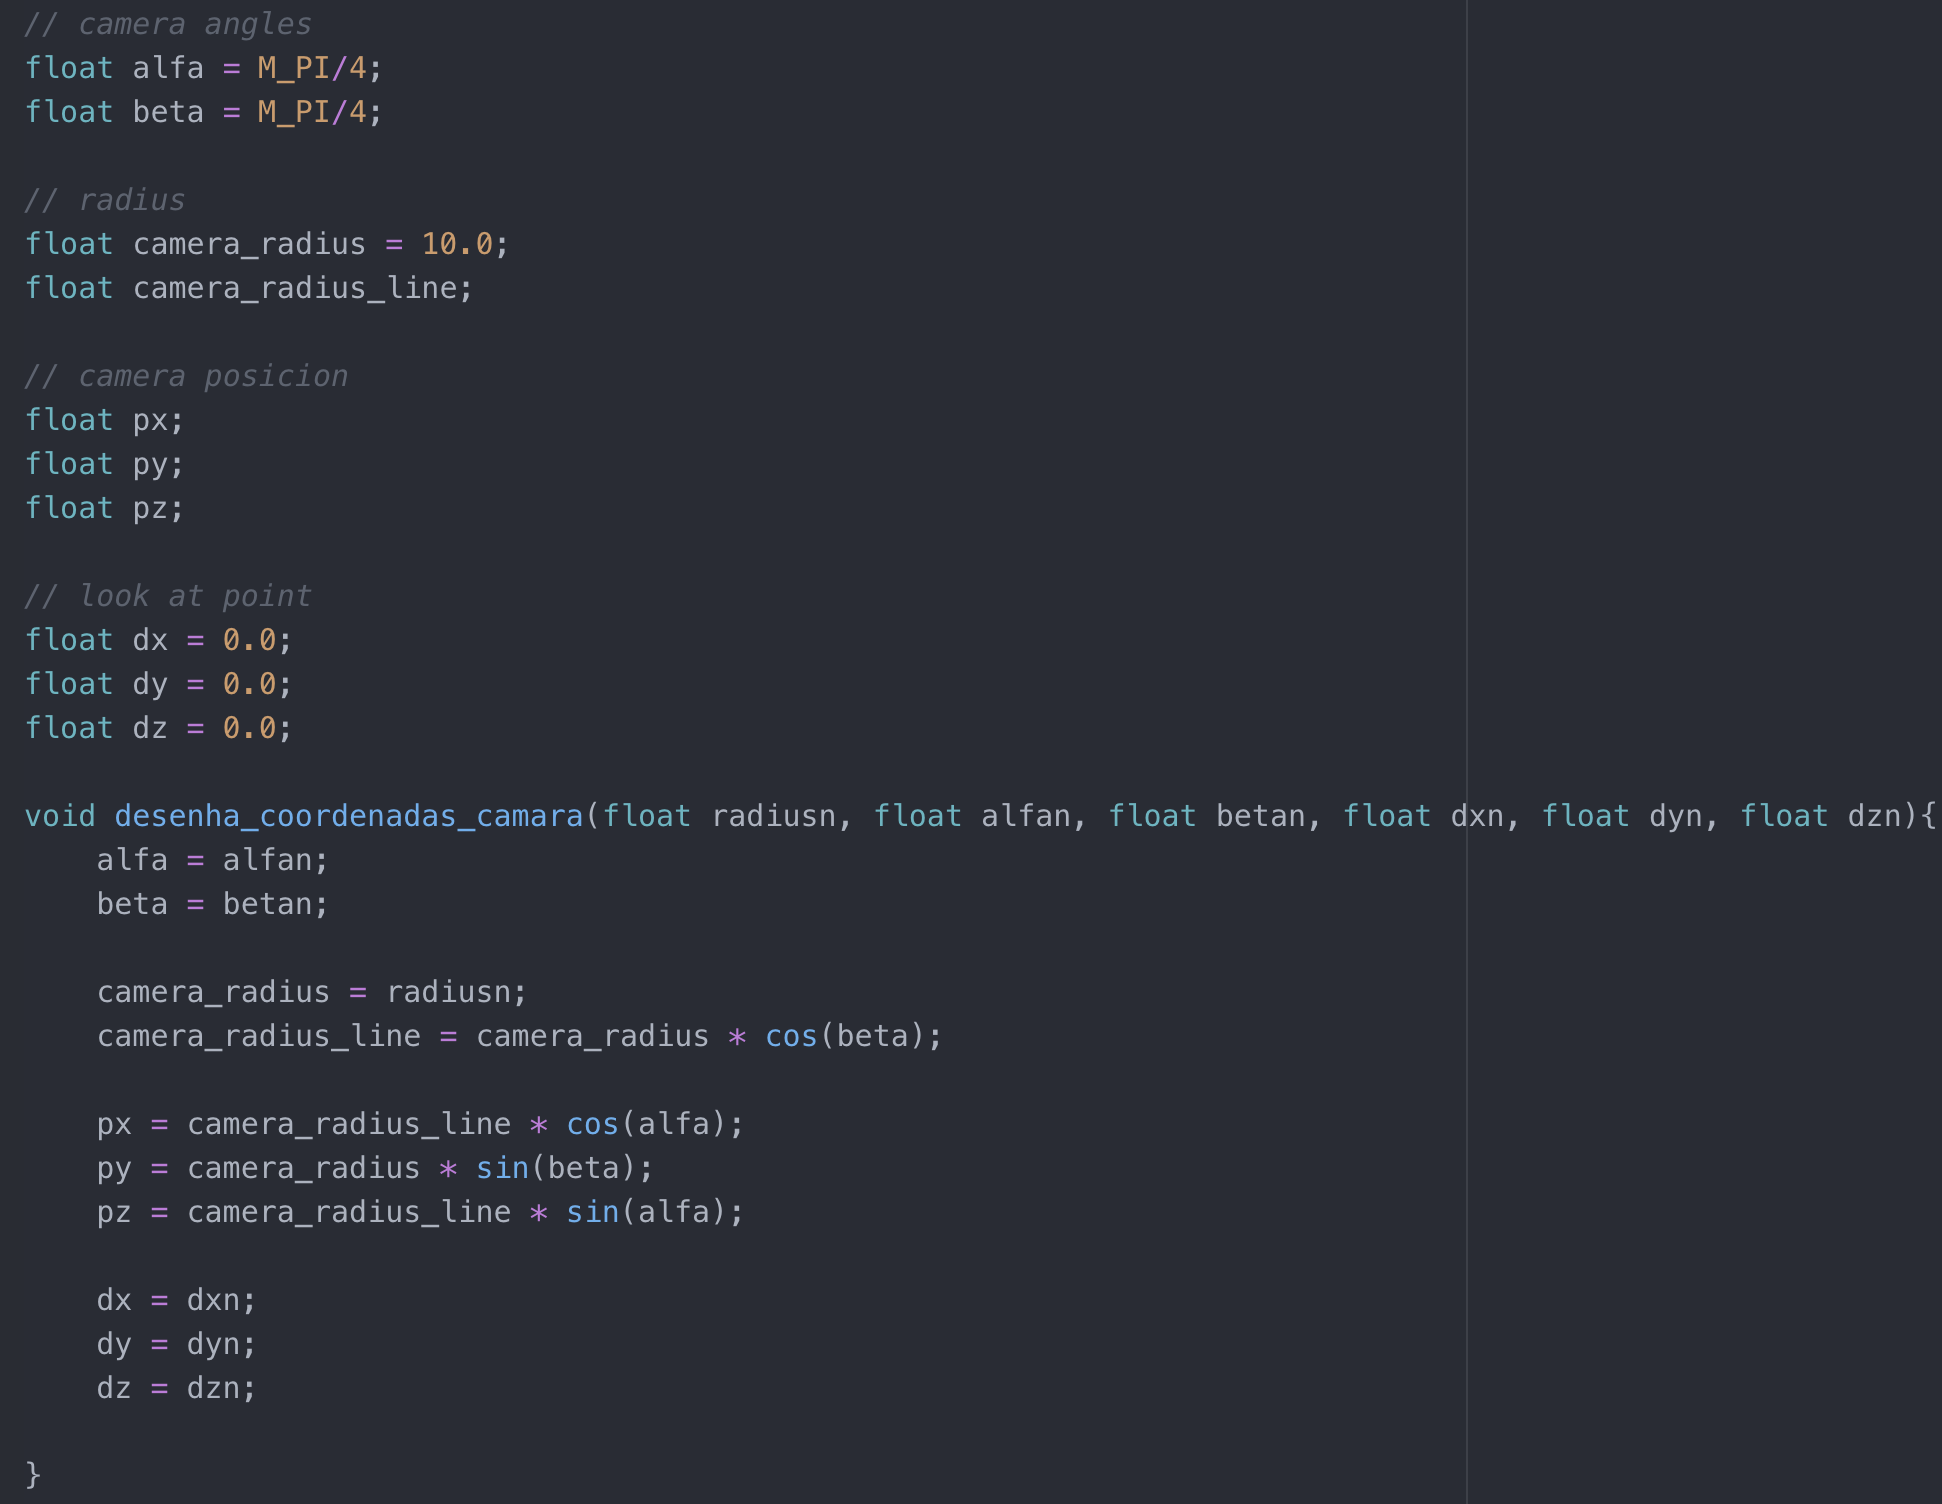
\includegraphics[scale=0.40]{funcao_desenha.png}
\caption{Função encarregue dos parâmetros da câmara.}
\label{img:desenha}
\end{figure}

Como é descrito na figura \ref{img:desenha}, realizamos uma função que está encarregue de atualizar e gerir todos os parâmetros referentes à câmera. Esta função é realizada consoante qualquer alteração num destes parâmetros.

Por forma a envolver diretamente estes parâmetros com a câmera, inserimo-los na função \emph{gluLookAt()}, como é possível visualizar na figura \ref{img:glulookat}.

\begin{figure}[H]
\centering
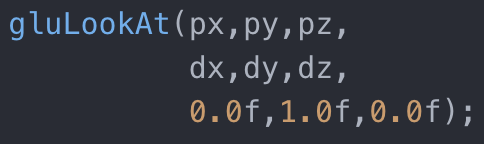
\includegraphics[scale=0.70]{gluLookAt.png}
\caption{Função que contém a matriz da câmera.}
\label{img:glulookat}
\end{figure}

A câmera é também um mecanismo muito forte de deteção de erros, uma vez que nos permite visualizar as figuras de várias formas e perspetivas.


\section{Conclusão}
\label{sec:conclusao}




\end{document}
